\subsection{Cost Function}
\label{sec:cost_function}

In this paper, we define AAM fitting as the \emph{regularized} search over the shape and appearance parameters that minimize a global measure of similarity between the vectorized warped image and the appearance model:
\begin{equation}
    \begin{aligned}
        \mathbf{p}^*, \mathbf{c}^* & = \underset{\mathbf{p}, \mathbf{c}} {\mathrm{arg\, min\;}} \mathcal{R} (\mathbf{p}, \mathbf{c}) + \mathcal{D} (\mathbf{i}[\mathbf{p}], \mathbf{c}) 
        \end{aligned}
    \label{eq:aam_fitting}
\end{equation}
where $\mathcal{R}$ is a regularization term that penalizes complex shape and appearance deformations and $\mathcal{D}$ is a data term that
quantifies the global measure of similarity between the vectorized warped image and the appearance model.

\subsubsection{Regularized Sum of Squared Differences}
\label{sec:rssd}

Arguably, the most natural choices for the previous data and regularization terms are the SSD between the vectorized warped image and the linear appearance model\footnote{This choice of $\mathcal{D}$ is very related to the second main assumption behind AAMs, Equation \ref{eq:aam_2}.} and the sum of $\l_2^2$-norms over the shape and appearance parameters respectively:
\begin{equation}
    \begin{aligned}
        \mathbf{p}^*, \mathbf{c}^* & = \underset{\mathbf{p}, \mathbf{c}} {\mathrm{arg\, min\;}} \underbrace{\frac{1}{2}||\mathbf{p}||^2 + \frac{1}{2}||\mathbf{c}||^2}_{\mathcal{R} (\mathbf{p}, \mathbf{c})} +
        \\
        & \qquad \qquad \quad \underbrace{\frac{1}{2}|| \mathbf{i}[\mathbf{p}] - (\mathbf{\bar{a}} + \mathbf{A} \mathbf{c}) ||^2}_{\mathcal{D} (\mathbf{i}[\mathbf{p}], \mathbf{c})}
    \end{aligned}
    \label{eq:rssd}
\end{equation}
\subsubsection*{Probabilistic Formulation}
\label{sec:rssd_pi}

A probabilistic interpretation of the previous cost function can be naturally derived using the probabilistic generative models introduced in Section \ref{sec:probabilistic_aam}. Denoting the models' parameters as \mbox{$\Theta = \{\mathbf{\bar{s}}, \mathbf{S}, \mathbf{\Lambda}, \mathbf{\bar{a}}, \mathbf{A}, \mathbf{\Sigma}, \sigma^2\}$} and taking into account the prior distributions over the shape and texture parameters:
\begin{equation}
    \begin{aligned}
        \mathbf{p}^*, \mathbf{c}^* & = \underset{\mathbf{p}, \mathbf{c}}{\mathrm{arg\,max\;}} p(\mathbf{p}, \mathbf{c}, \mathbf{i}[\mathbf{p}] | \Theta) 
        \\
        & = \underset{\mathbf{p}, \mathbf{c}}{\mathrm{arg\,max\;}}  p(\mathbf{p} | \mathbf{\Lambda})  p(\mathbf{c} | \mathbf{\Sigma}) p(\mathbf{i}[\mathbf{p}] |
        \mathbf{p}, \mathbf{c}, \Theta)  
        \\
        & = \underset{\mathbf{p}, \mathbf{c}}{\mathrm{arg\,max\;}}  \ln p(\mathbf{p} | \mathbf{\Lambda}) + \ln p(\mathbf{c} | \mathbf{\Sigma}) +
        \\
        & \qquad \qquad \quad \ln p(\mathbf{i}[\mathbf{p}] | \mathbf{p}, \mathbf{c}, \Theta)
        \\
        & = \underset{\mathbf{p}, \mathbf{c}}{\mathrm{arg\,min\;}}  \underbrace{\frac{1}{2} ||\mathbf{p}||^2_{\mathbf{\Lambda}^{-1}} + \frac{1}{2}||\mathbf{c}||^2_{\mathbf{\Sigma}^{-1}}}_{\mathcal{R}(\mathbf{p}, \mathbf{c})} +
        \\
        & \qquad \qquad \quad \underbrace{ \frac{1}{2\sigma^2} || \mathbf{i}[\mathbf{p}] - (\mathbf{\bar{a}} + \mathbf{A} \mathbf{c}) ||^2}_{\mathcal{D}(\mathbf{i}[\mathbf{p}], \mathbf{c})} 
    \end{aligned}
    \label{eq:prob_rssd}
\end{equation}
where we have assumed the shape and appearance parameters to be independent\footnote{This is a common assumption in CGD algorithms \cite{Matthews2004}, however, in reality, some degree of dependence between these parameters is to be expected \cite{Cootes2001}.}.

The previous Maximum-A-Posteriori (MAP) formulation is a weighted version of the optimization problem defined by Equation \ref{eq:rssd}. The maximization of the prior probability over the shape and texture parameters leads to the minimization of the regularization term $\mathcal{R}$ and the maximization of the conditional probability of the vectorized warped image given the shape, texture and model parameters leads to the minimization of the data term $\mathcal{D}$.

\subsubsection{Regularized Project-Out}
\label{sec:rpo}

Matthews and Baker showed in \cite{Matthews2004} that one could express the SSD between the vectorized warped image and the linear appearance model (Equation \ref{eq:ssd}) as the sum of two different terms:
\begin{equation}
    \begin{aligned}
        \frac{1}{2}\mathbf{r}^T \mathbf{r} & = \frac{1}{2}\mathbf{r}^T (\mathbf{A}\mathbf{A}^T + \mathbf{I} - \mathbf{A}\mathbf{A}^T) \mathbf{r}
        \\
        & = \frac{1}{2}\mathbf{r}^T (\mathbf{A}\mathbf{A}^T) \mathbf{r} + \frac{1}{2}\mathbf{r}^T (\mathbf{I} - \mathbf{A}\mathbf{A}^T) \mathbf{r}
        \\
        & = \frac{1}{2}\left\| \mathbf{i}[\mathbf{p}] - \left( \bar{\mathbf{a}} + \mathbf{A} \mathbf{c} \right) \right\|_{\mathbf{A}\mathbf{A}^T}^2 \, + 
        \\
        & \quad \, \frac{1}{2}\left\| \mathbf{i}[\mathbf{p}] - \left( \bar{\mathbf{a}} + \mathbf{A} \mathbf{c} \right) \right\|_{\mathbf{I} - \mathbf{A}\mathbf{A}^T}^2 
        \\
        & = f_1(\mathbf{p}, \mathbf{c}) + f_2(\mathbf{p}, \mathbf{c})
    \label{eq:ssd_terms}
    \end{aligned}
\end{equation}
The first term defines the distance \emph{within} the appearance subspace and it is always $0$ regardless of the value of the shape parameters $\mathbf{p}$:
\begin{equation}
    \begin{aligned}
        f_1(\mathbf{p}, \mathbf{c}) & = \frac{1}{2}\left\| \mathbf{i}[\mathbf{p}] - \left( \bar{\mathbf{a}} + \mathbf{A} \mathbf{c} \right) \right\|_{\mathbf{A}\mathbf{A}^T}^2
        \\
        & = \frac{1}{2} \left( \underbrace{\mathbf{i}[\mathbf{p}]^T \mathbf{A}}_{\mathbf{c}^T} \underbrace{\mathbf{A}^T \mathbf{i}[\mathbf{p}]}_{\mathbf{c}} - \underbrace{2\overbrace{\mathbf{i}[\mathbf{p}]^T \mathbf{A}}^{\mathbf{c}^T} \overbrace{\mathbf{A}^T \bar{\mathbf{a}}}^{\mathbf{0}}}_{0} \, - \right.
        \\
        & \quad \,\, 2\underbrace{\mathbf{i}[\mathbf{p}]^T \mathbf{A}}_{\mathbf{c}^T} \underbrace{\overbrace{\mathbf{A}^T \mathbf{A}}^{\mathbf{I}} \mathbf{c}}_{\mathbf{c}} + \underbrace{\overbrace{\bar{\mathbf{a}}^T \mathbf{A}}^{\mathbf{0}^T} \overbrace{\mathbf{A}^T \bar{\mathbf{a}}}^{\mathbf{0}}}_{0} \, +
        \\
        & \quad \,\, \left. \underbrace{\mathbf{c}^T \overbrace{\mathbf{A}^T \mathbf{A}}^{\mathbf{I}}}_{\mathbf{c}^T} \underbrace{\overbrace{\mathbf{A}^T \mathbf{A}}^{\mathbf{I}} \mathbf{c}}_{\mathbf{c}} \right)
        \\
        & = \frac{1}{2}(\mathbf{c}^T\mathbf{c} - 2\mathbf{c}^T\mathbf{c} + \mathbf{c}^T\mathbf{c})
        \\
        & = 0
    \label{eq:ssd_term1}
    \end{aligned}
\end{equation}
The second term measures the distance \emph{to} the appearance subspace i.e. the distance within its orthogonal complement. After some algebraic manipulation, one can show that this term reduces to a function that only depends on the shape parameters $\mathbf{p}$:
\begin{equation}
    \begin{aligned}
        f_2(\mathbf{p}, \mathbf{c}) & = \frac{1}{2}\left\| \mathbf{i}[\mathbf{p}] - \left( \bar{\mathbf{a}} + \mathbf{A} \mathbf{c} \right) \right\|_{\bar{\mathbf{A}}}^2
        \\
        & = \frac{1}{2} \left( \mathbf{i}[\mathbf{p}]^T \bar{\mathbf{A}} \mathbf{i}[\mathbf{p}] - 2\mathbf{i}[\mathbf{p}]^T \bar{\mathbf{A}} \bar{\mathbf{a}} \, - \right.
        \\
        & \quad \,\, \left. \underbrace{2\mathbf{i}[\mathbf{p}]^T \bar{\mathbf{A}} \mathbf{A}\mathbf{c}}_{0} + \bar{\mathbf{a}}^T \bar{\mathbf{A}} \bar{\mathbf{a}} + \underbrace{\mathbf{c}^T \mathbf{A}^T \bar{\mathbf{A}} \mathbf{A}\mathbf{c}}_{0} \right)
        \\
        & = \frac{1}{2} (\mathbf{i}[\mathbf{p}]^T \bar{\mathbf{A}} \mathbf{i}[\mathbf{p}] - 2\mathbf{i}[\mathbf{p}]^T \bar{\mathbf{A}} \bar{\mathbf{a}} + \bar{\mathbf{a}}^T \bar{\mathbf{A}} \bar{\mathbf{a}} )
        \\
        & = \frac{1}{2} \left\| \mathbf{i}[\mathbf{p}] - \bar{\mathbf{a}} \right\|_{\bar{\mathbf{A}}}^2
    \label{eq:ssd_term2}
    \end{aligned}
\end{equation}
where, for convenience, we have defined the orthogonal complement to the appearance subspace as $\bar{\mathbf{A}}= \mathbf{I} -\mathbf{A}\mathbf{A}^T$. Note that, as mentioned above, the previous term does not depend on the appearance parameters $\mathbf{c}$:
\begin{equation}
    \begin{aligned}
        f_2(\mathbf{p}, \mathbf{c}) & = \hat{f}_2(\mathbf{p}) = \frac{1}{2}\left\| \mathbf{i}[\mathbf{p}] - \bar{\mathbf{a}} \right\|_{\bar{\mathbf{A}}}^2
    \label{eq:po}
    \end{aligned}
\end{equation}

Therefore, using the previous \emph{project-out trick}, the minimization problem defined by Equation \ref{eq:rssd} reduces to:
\begin{equation}
    \begin{aligned}
        \mathbf{p}^* & = \underset{\mathbf{p}} {\mathrm{arg\, min\;}} \underbrace{\frac{1}{2}||\mathbf{p}||^2}_{\mathcal{R} (\mathbf{p})} + \underbrace{\frac{1}{2}|| \mathbf{i}[\mathbf{p}] - \mathbf{\bar{a}} ||^2_{\bar{\mathbf{A}}}}_{\mathcal{D} (\mathbf{i}[\mathbf{p}])}
    \label{eq:rpo}
    \end{aligned}
\end{equation}

\subsubsection*{Probabilistic Formulation}
\label{sec:po_pi}
In our preliminary work \cite{Alabort2014}, we showed that assuming the probabilistic models defined in Section \ref{sec:probabilistic_aam} a Bayesian version of the previous project-out data term could be naturally derived by marginalizing over the appearance parameters to obtain the following marginalized density:
\begin{equation}
    \begin{aligned}
        p(\mathbf{i}[\mathbf{p}] | \mathbf{p}, \Theta) & = \int_c p(\mathbf{i}[\mathbf{p}] | \mathbf{p}, \mathbf{c}, \Theta) p(\mathbf{c}|\mathbf{\Sigma}) d\mathbf{c} 
        \\
        & = \mathcal{N}(\bar{\mathbf{a}}, \mathbf{A}\mathbf{\Sigma}\mathbf{A}^T + \sigma^2 \mathbf{I})
    \end{aligned}
    \label{eq:marginal}
\end{equation}
and using the Woodbury formula\footnote{
\begin{equation*}
    \begin{aligned}
    \small
    	(\mathbf{A} \mathbf{\Sigma} \mathbf{A}^T + \sigma^2 \mathbf{I})^{-1} & = \frac{1}{\sigma^2} \mathbf{I} - \frac{1}{\sigma^4} \mathbf{A} \underbrace{(\mathbf{\Sigma}^{-1} + \frac{1}{\sigma^2}\mathbf{I})^{-1}}_{\textrm{reapply Woodbury}} \mathbf{A}^T
    	\\
    	& = \frac{1}{\sigma^2} \mathbf{I} - \frac{1}{\sigma^4} \mathbf{A} (\sigma^2\mathbf{I} - \sigma^4(\mathbf{\Sigma + \sigma^2\mathbf{I}})^{-1}) \mathbf{A}^T
    	\\
    	& = \frac{1}{\sigma^2} \mathbf{I} - \frac{1}{\sigma^4} \mathbf{A} (\sigma^2\mathbf{I} - \sigma^4\mathbf{D}^{-1}) \mathbf{A}^T
    	\\
    	& = \mathbf{A}\mathbf{D}^{-1}\mathbf{A}^T + \frac{1}{\sigma^2} (\mathbf{I} - \mathbf{A}\mathbf{A}^T)
    \end{aligned}
    \label{eq:woodbury}
\end{equation*}} \cite{Woodbury1950} to decompose the logarithm of the previous density into the sum of two different terms:
\begin{equation}
    \begin{aligned}
        \ln p(\mathbf{i}[\mathbf{p}] | \mathbf{p}, \Theta) & = \frac{1}{2}|| \mathbf{i}[\mathbf{p}] - \mathbf{\bar{a}} ||^2_{(\mathbf{A}\mathbf{\Sigma}\mathbf{A}^T + \sigma^2 \mathbf{I})^{-1}}
        \\
        & = \frac{1}{2}|| \mathbf{i}[\mathbf{p}] - \mathbf{\bar{a}} ||^2_{\mathbf{A}\mathbf{D}^{-1}\mathbf{A}^T} + 
        \\
        & \quad \, \frac{1}{2\sigma^2}|| \mathbf{i}[\mathbf{p}] - \mathbf{\bar{a}} ||^2_{\bar{\mathbf{A}}}
    \end{aligned}
    \label{eq:prob_po}
\end{equation}
where $\mathbf{D} = \textrm{diag}[\lambda_1 + \sigma^2, \cdots, \lambda_m + \sigma^2]$.

As depict by Figure \ref{fig:bayes}, the previous two terms define respectively: 
\begin{inparaenum}[\itshape i\upshape)]
    \item the Mahalanobis distance \emph{within} the linear appearance subspace; and 
    \item the Euclidean distance \emph{to} the linear appearance subspace (i.e. the Euclidean distance within its orthogonal complement) weighted by the inverse of the estimated image noise.
\end{inparaenum} 
Note that when the variance $\mathbf{\Sigma}$ of the prior distribution over the latent appearance space increases (and especially as
$\mathbf{\Sigma} \rightarrow \infty$) $\mathbf{c}$ becomes uniformly distributed and the contribution of the first term $\frac{1}{2}|| \mathbf{i}[\mathbf{p}] - \mathbf{\bar{a}} ||^2_{\mathbf{A}\mathbf{D}^{-1}\mathbf{A}^T}$ vanishes and we obtain a weighted version of the project-out data term defined by Equation \ref{eq:po}. 

A MAP formulation with respect to the shape parameters for the previous Bayesian interpretation of the project-out cost function can be derived as follows:
\begin{equation}
    \begin{aligned}
        \mathbf{p}^* & = \underset{\mathbf{p}}{\mathrm{arg\,max\;}} p(\mathbf{p}, \mathbf{i}[\mathbf{p}] | \Theta) 
        \\
        & = \underset{\mathbf{p}}{\mathrm{arg\,max\;}}  p(\mathbf{p} | \mathbf{\Lambda})  p(\mathbf{i}[\mathbf{p}] |
        \mathbf{p}, \Theta)  
        \\
        & = \underset{\mathbf{p}}{\mathrm{arg\,max\;}}  \ln p(\mathbf{p} | \mathbf{\Lambda}) + \ln p(\mathbf{i}[\mathbf{p}] | \mathbf{p}, \Theta)
        \\
        & = \underset{\mathbf{p}}{\mathrm{arg\,min\;}}  \underbrace{\frac{1}{2} ||\mathbf{p}||^2_{\mathbf{\Lambda}^{-1}}}_{\mathcal{R}(\mathbf{p})} + \underbrace{\frac{1}{2\sigma^2}|| \mathbf{i}[\mathbf{p}] - \mathbf{\bar{a}} ||^2_{\mathbf{Q}}}_{\mathcal{D}(\mathbf{i}[\mathbf{p}])}
    \end{aligned}
    \label{eq:prob_rpo}
\end{equation}
where we have defined the Bayesian project-out operator as $\mathbf{Q} = \mathbf{I} - \mathbf{A}(\mathbf{I} - \sigma^2\mathbf{D}^{-1})\mathbf{A}^T$.

\begin{figure}
    \centering
    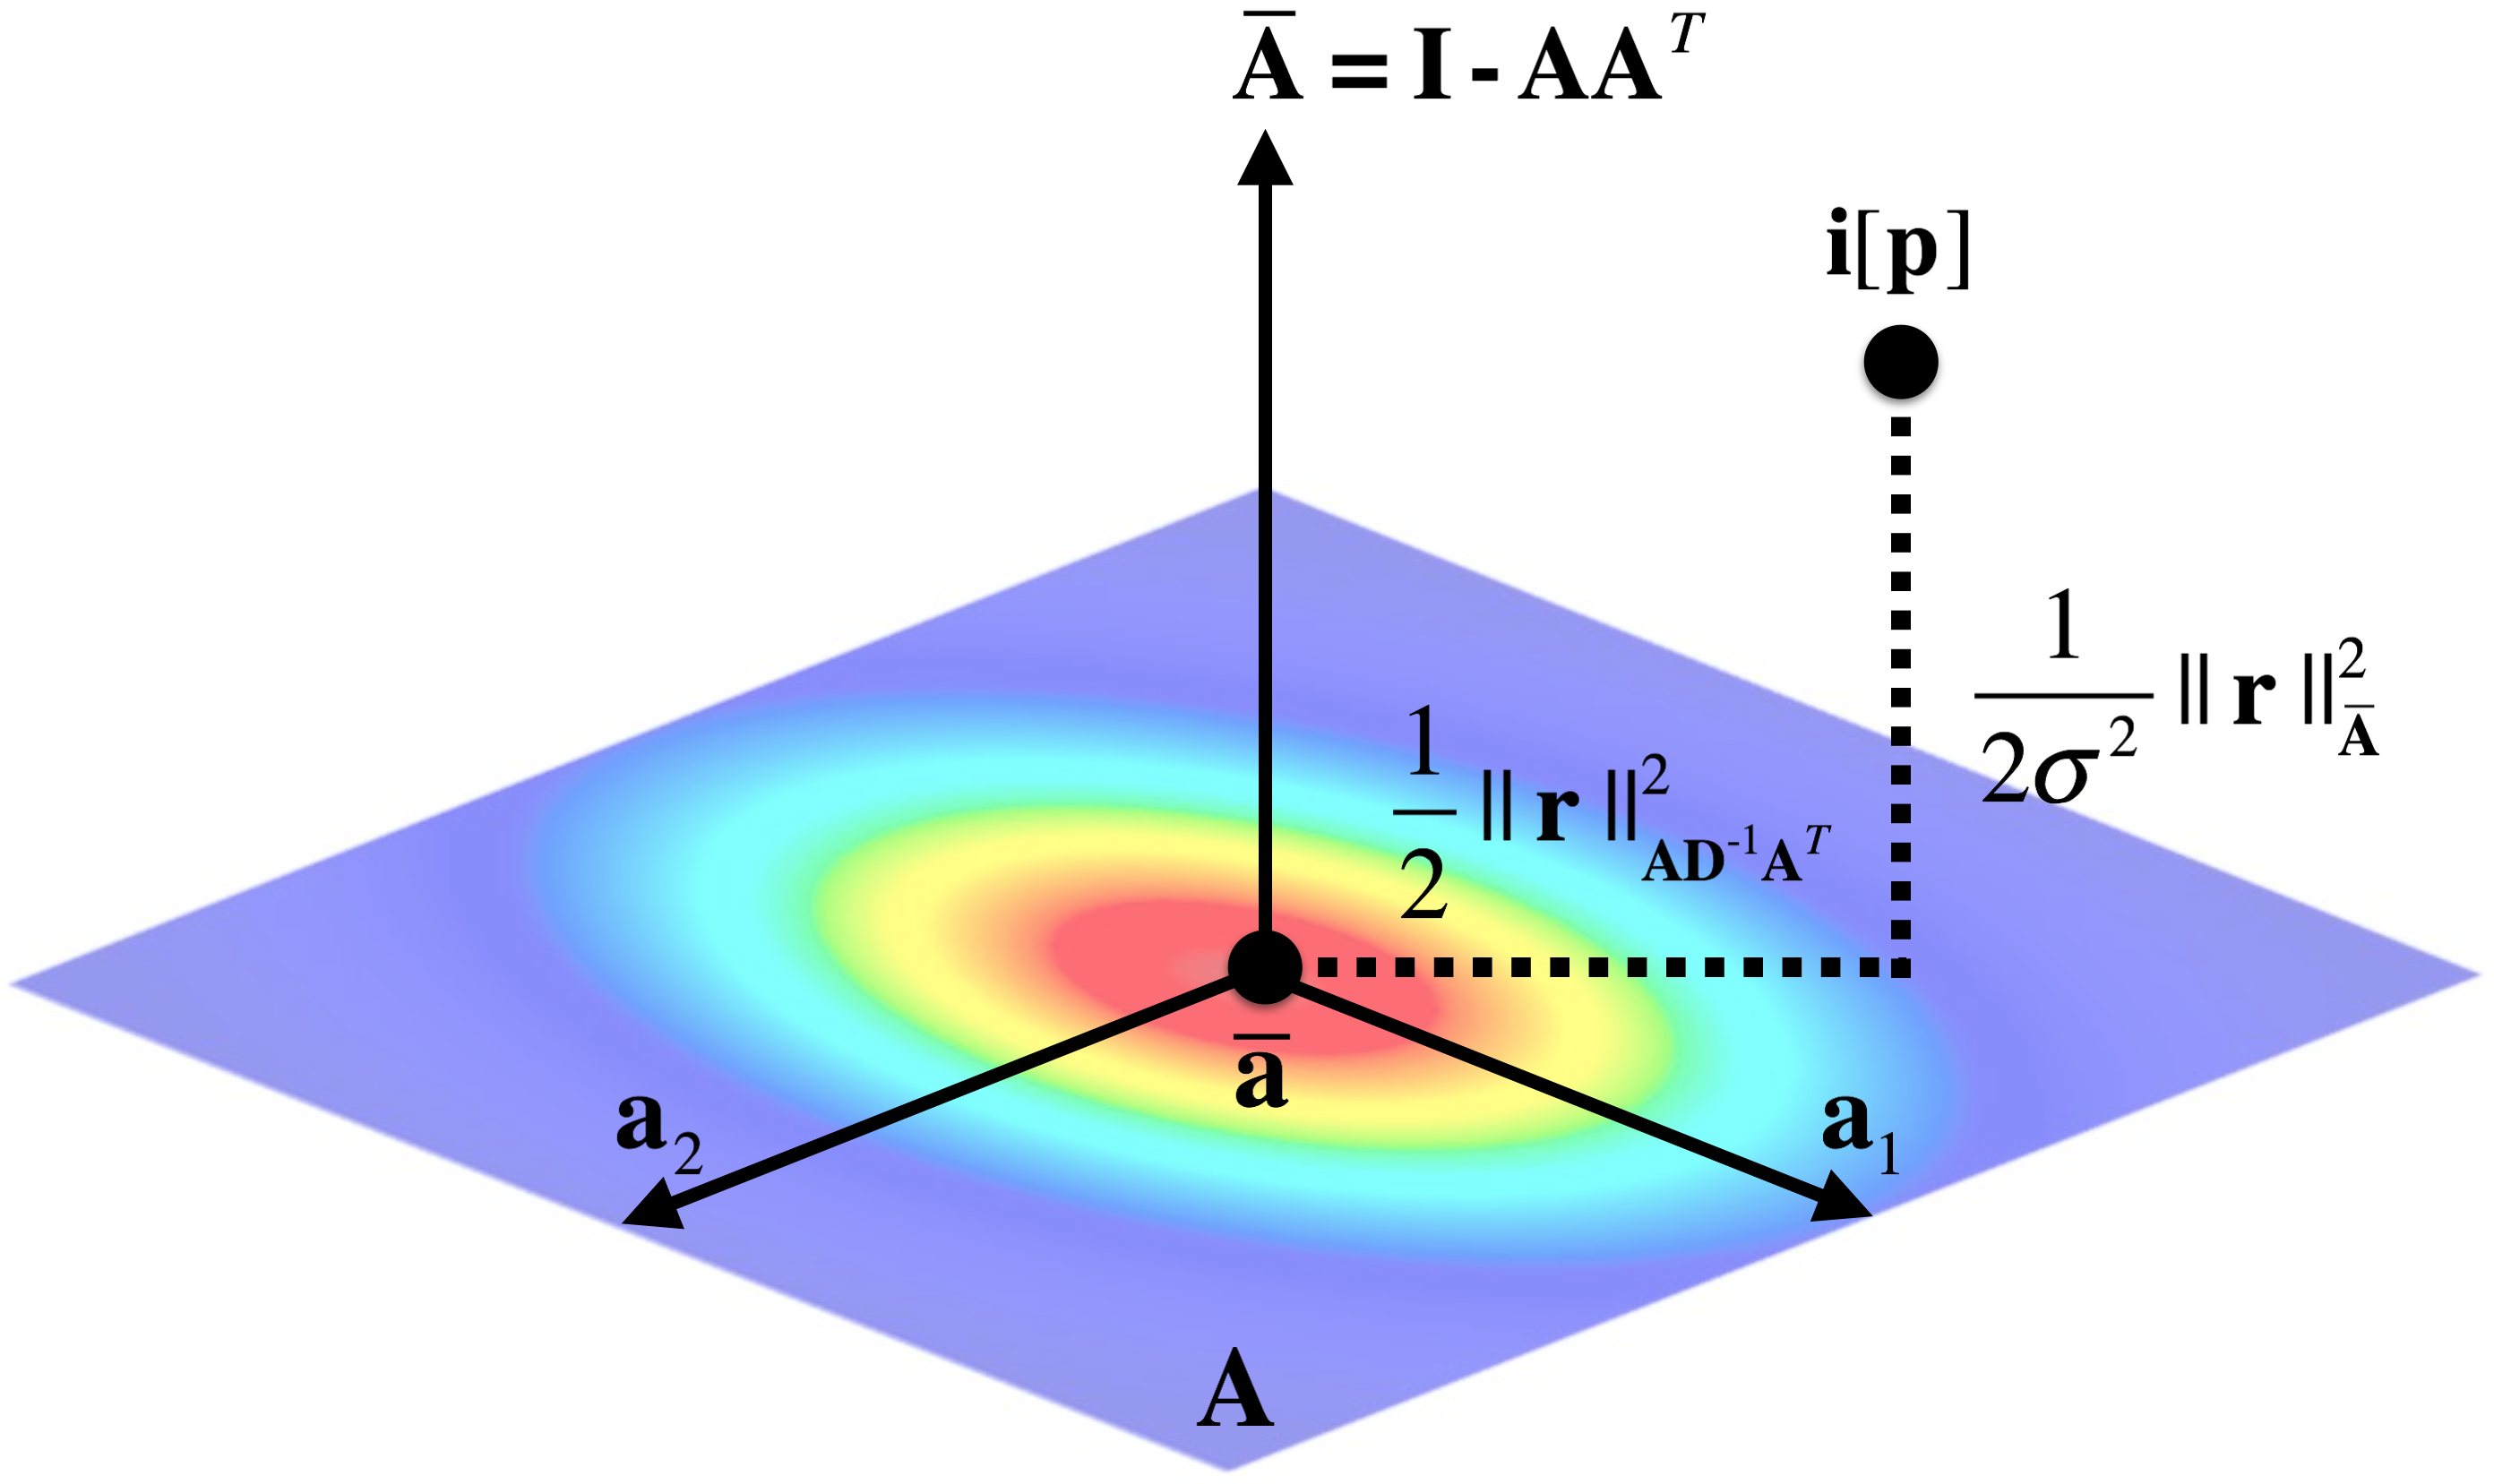
\includegraphics[width=0.50\textwidth]{figures/bayes.png}
    \caption{The Bayesian project-out formulation fits AAMs by minimiz- ing two different distances: $i)$ the Mahalanobis distance \emph{within} the linear appearance subspace; and $ii)$ the Euclidean distance \emph{to} the linear appearance subspace (i.e. the Euclidean distance within its orthogonal complement) weighted by the inverse of the estimated image noise.}
    \label{fig:bayes}
\end{figure}
